\section{Supplementary protocols and controls}\label{sec:supp}
\subsection{Source-training variants}
For the earlier submitted training variant, each iteration added prefix supervision with probability 0.5, drawing the fraction uniformly from $[0.1,1]$ on that branch. Section~\ref{sec:method} specifies the discrete schedule for the prefix-supervised sources used in the ranking comparisons.
\subsection{Validation against physical single-point deletion}
We compared the predicted RGB mean squared error (MSE) with the change in the display renderer after physically removing one point. For Cut seed zero we used four training observations, stratified by score rank and supplemented with points where C and U disagreed. The matched analysis comprises 96 point--view pairs from 68 distinct canonical point IDs. Every ID in these pairs belongs to the 15\% U subset. Removing the same ID in the full source and in that subset therefore defines both measurements. Each context has 28 pairs with exactly zero measured perturbation. Repeated views of the same point are not independent replicates.

Over all 96 pairs, the pooled Spearman correlation was 0.9985 in the full source. In the reduced context, the full-source score gave 0.9609 and the score recomputed in the subset gave 0.9986. To assess magnitude, among the 68 pairs per context with measured MSE above $10^{-15}$, the median predicted-to-measured ratio was 1.000 in both contexts. The 10th--90th percentile intervals were 0.963--1.007 (full) and 0.959--1.016 (subset). Figure~\ref{fig:deletion_check} shows the individual errors. These comparisons validate single-point perturbations on the sampled views. The PSNR comparisons between complete pruning schedules measure the effect of removing many points together.
\begin{figure}[htbp]\centering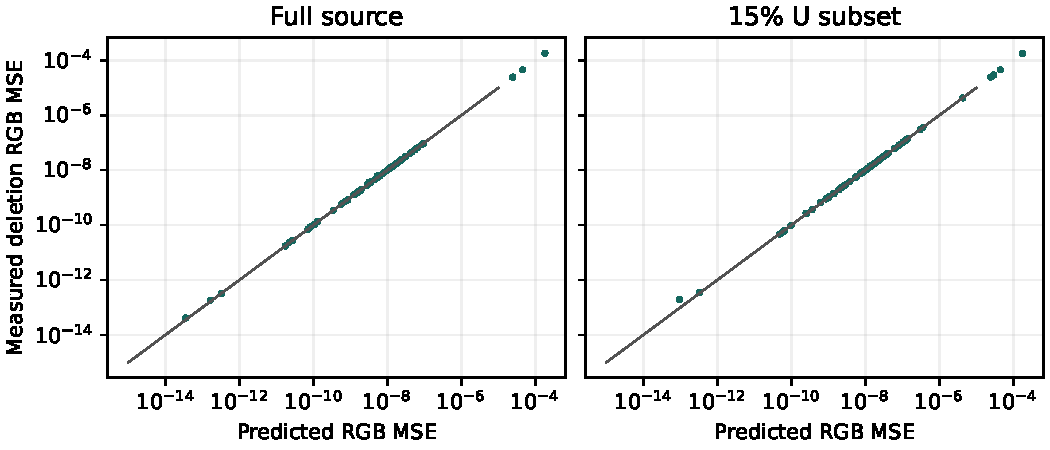
\includegraphics[width=.94\linewidth]{deletion_magnitude.pdf}
\caption{Predicted and measured MSE in each point's current rendering context. Only pairs with both values positive appear on logarithmic axes. The diagonal denotes equal predicted and measured errors.}\label{fig:deletion_check}\end{figure}
\subsection{Calibration coverage across time}
On the prepared scenes, the calibration procedure selects equally spaced ranks among the available training times and cycles among the cameras available at those times. On Cut seed zero, we varied the observation count (8, 16, 32 and 64) and the initial camera offset (0, 6 and 12). At 10\% retention, C yielded 29.765--29.944~dB using eight observations, 30.058--30.138~dB using 32, and 30.075--30.117~dB using 64. Figure~\ref{fig:time_cut} shows the framewise comparison for the original 32 observations.
\begin{figure}[htbp]\centering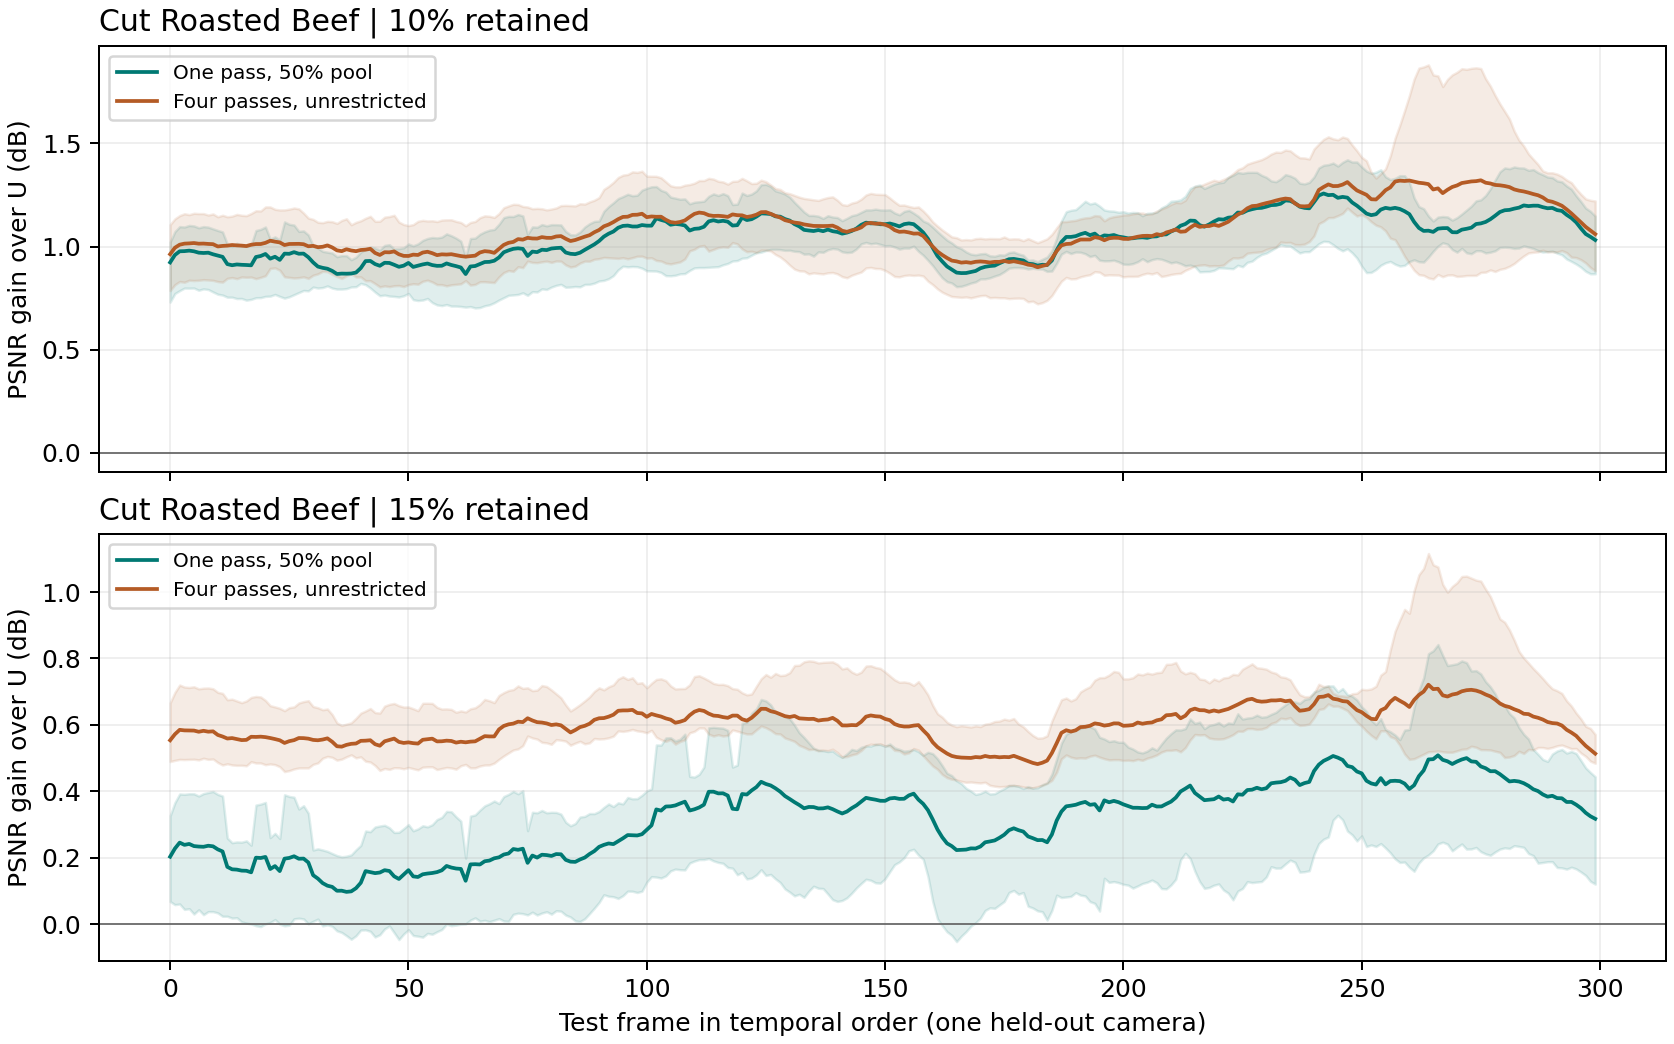
\includegraphics[width=\linewidth]{temporal.png}
\caption{Quality relative to one unrestricted pass, in the temporal order of the 300 held-out Cut frames. Lines show means across three prefix-supervised sources. Shading spans the three source values per frame.}\label{fig:time_cut}\end{figure}

\subsection{Comparing two rankings across 13 real scenes at 25\% retention}
\label{sec:historical}
Table~\ref{tab:historical} compares opacity and protected-core rankings at 25\% retention across 13 real scenes from three dataset families. Each row uses one source checkpoint and reports the endpoint after 2,000 fine-tuning steps on both opacity (O) and protected-core (P) subsets. P gains in 11 scenes, by at least 0.5~dB in five and at least 1~dB in one. Gains are small in the NeRF-DS scenes and two of those pairs favor O. Table~\ref{tab:sourcefilter} compares C and U across two source families in eight paired scenes. The budget and adaptation experiments use four prefix-supervised scenes with three sources each.

\begin{table*}[t]
\centering\small
\caption{Opacity and protected-core rankings at 25\% retention after 2,000 matched fine-tuning steps, with one source per scene. Absolute PSNR and paired differences are in dB.}
\label{tab:historical}
\begin{tabular}{llrrr}
\hline
Dataset & Scene & O & P & P--O \\
\hline
\resultrows{results_assets/historical.tex}
\hline
\end{tabular}
\end{table*}

\subsection{Independent fixed-capacity training}
\label{sec:capacity}
We also evaluate a model trained separately for each of two 25\% targets (Chicken and Cut, one source per scene). Each run trains for 33,000 updates with a Gaussian capacity constraint during densification and reaches its target exactly. O, P and C use cold subsets of the corresponding existing source at that identical count. The cold C subset exceeds the matched capacity model by 2.02~dB on Chicken and 0.15~dB on Cut. The independently trained model is 1.92~dB below P on Chicken and 0.10~dB below P on Cut. On Cut, independent training has better SSIM (0.931 versus 0.924 for P), while P has lower LPIPS (0.071 versus 0.089). The independent capacity runs took 910.4 and 938.7 seconds on Chicken and Cut, using full-only supervision plus native regularization. The corresponding reusable sources took 2,159 and 2,226 seconds with full and prefix supervision. Each trained source supplies all five cold budgets from the same weights.

\begin{table*}[t]
\centering\small
\caption{Independent 25\% fixed-capacity training control. Each comparison uses the same target count $K$ and matched test views. Training seconds refer to the separately trained capacity model's training loop. Quality is PSNR (dB).}
\label{tab:capacity}
\setlength{\tabcolsep}{3pt}\begin{tabular}{lrrrrrr}
\hline
Scene & $K$ & Fixed capacity & Cold O & Cold P & Cold C & Train (s) \\
\hline
\resultrows{results_assets/capacity.tex}
\hline
\end{tabular}
\end{table*}

\subsection{Comparison with opacity times scale area}
For comparison we also evaluate an earlier opacity--scale product. Its implementation uses
\begin{equation}
s_i^{\mathrm{legacy}}(t)
=\operatorname{sigmoid}(\widetilde o_i(t))\,
s_{ix}^{\mathrm{can}}s_{iy}^{\mathrm{can}},
\label{eq:legacy-score}
\end{equation}
where $\widetilde o_i(t)$ is the opacity logit returned by the deformation module and $s_{ix}^{\mathrm{can}}$ and $s_{iy}^{\mathrm{can}}$ are activated canonical scale components. Opacity deformation is disabled in the archived comparison configurations, so the product is time invariant there. The two scale components are in canonical coordinates. The main comparison uses the rendering-based score in Eq.~\eqref{eq:deletion-score}.


\subsection{Ranking within a fixed opacity band}\label{sec:bridge}
An earlier matched experiment held the opacity core, candidate band, source and count fixed and changed the ordering within the band. The comparators used the opacity--scale product in Eq.~\eqref{eq:legacy-score}, one frozen random order per source, or a feedback-based protected ordering (H). The first two controls isolate the contribution of the ranking within the same band. H also changes the calibration procedure.
\begin{table}[htbp]
\centering
\caption{Effect of changing the ranking within the protected band at 25\% retention. Each entry is the mean paired difference in cold PSNR (P minus comparator, dB) across three sources. Positive values favor P.}\label{tab:scorebridge}
\begin{tabular}{lrrr}
\toprule
Scene & Opacity--scale & Random order & Feedback (H) \\
\midrule
Chicken & +3.0496 & +2.6040 & -0.0418 \\
Cut roasted beef & +2.1925 & +2.4405 & -0.0331 \\
Sear steak & +2.1149 & +2.2713 & -0.0305 \\
Basin & +0.0133 & +0.0750 & +0.0003 \\
\bottomrule
\end{tabular}
\end{table}

P outperformed the opacity--scale product and the fixed random order on all twelve sources. Feedback yielded higher PSNR than P on eleven. The latter improvement adds an offline cost: on Chicken, Cut roasted beef and Sear steak, the median selection time over three independent processes was 3.22--3.37 times as long for H as for P. Including loading and saving reduced the ratio to 1.49--1.57. These measurements compare the preparation cost of P and H only. Peak allocated memory during selection was higher for P.\par

\subsection{What remains visible at one quarter of the points}\label{sec:visual}
Figure~\ref{fig:visual} compares the same test view across the observation, the complete source, and three cold subsets. In all three frames, reranking recovers part of the quality lost under opacity truncation. We also compared the central $192\times144$ pixels against ground truth for all nine archived example views (three per scene, seed 0). In the 8-bit images, full-source crop PSNR exceeded cold C crop PSNR in all nine pairs, by 0.047--0.757~dB. The crop measurements quantify local reconstruction error, whereas the labels in the figure describe the entire frame.
\begin{figure}[htbp]
\centering
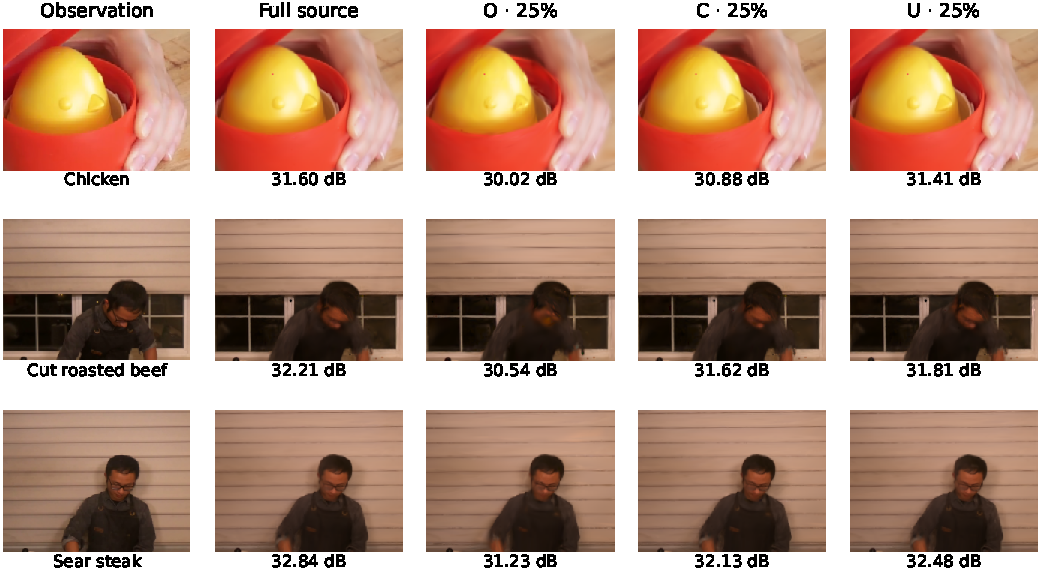
\includegraphics[width=\linewidth]{qualitative.pdf}
\caption{Matched central crops at 25\% retention. Each row uses seed 0 and the middle of three archived example views (source indices 165, 150, and 150, respectively). Each crop spans the central $192\times144$ native pixels. Values below the renderings give PSNR for the entire corresponding frame. The full-source column uses all points from the same source as the three subsets.}\label{fig:visual}
\end{figure}

For Press, a separate historical experiment on the protected-core order P contains 487 paired $240\times135$ test frames per seed across three seeds. At 25\% retention the mean full-minus-P PSNR gap is 0.018~dB, while the largest individual frame gap is 0.353~dB. These frame averages characterize the archived Press runs. The original figure used a separate rendering record.

\subsection{Model storage and transfer}\label{sec:delivery}
For each of the 12 sources, we serialized both the complete model and its cold C subset at 15\% retention. Both packages use an uncompressed archive of the native binary point cloud, deformation network, point-indexed deformation table, render settings and canonical point IDs. All 24 archives passed CPU round-trip checks. Removing points reduces the point-indexed payload while preserving the shared deformation network.
\begin{table}[htbp]
\centering\small
\caption{Payload size of complete and 15\% C models in decimal MB. Sizes are scene means over three checkpoints. Savings are the range of within-checkpoint reductions.}\label{tab:delivery}
\begin{tabular}{lrrr}\toprule
Scene & Full (MB) & C (MB) & Savings (\%) \\\midrule
Chicken & 78.15 & 37.08 & 51.3--53.3 \\
Cut Roasted Beef & 63.26 & 17.88 & 71.6--71.8 \\
Sear Steak & 59.97 & 17.39 & 70.7--71.4 \\
Basin & 76.16 & 48.41 & 36.4--36.5 \\\bottomrule
\end{tabular}
\end{table}
For Chicken seed 0 we served both packages over a loopback HTTP connection. The client received 75,314,041 bytes for the full model and 36,659,192 bytes for C, a 51.3\% reduction in response-body bytes. Both received files matched the source SHA-256 digests. This test measures the data to be delivered. Frame timings in Section~\ref{sec:runtime} were measured with the native RTX 3090 renderer.
At the same cold C 15\% membership and resident test cameras, rendering the materialized subset reduced peak PyTorch-allocated GPU memory by 29.0--47.0~MiB relative to gathering from the full model, across all 12 native RTX 3090 source pairs.

\subsection{Full-capacity comparison with independently trained standard 4DGS}\label{sec:basin_native}
For Basin, we compared standard 4DGS with the prefix-supervised source at each model's native full count. The three seed pairs shared the same initial point-cloud fingerprint within each pair. Each model received 17,000 training updates. We rendered the same 668 held-out frames at $240\times135$ on one RTX 3090, verified image and camera identities, and measured PSNR in a separate pass. For timing, we warmed up each model, synchronized each frame and alternated model order across three traversals and seeds. Both models rendered all of their primitives directly. Table~\ref{tab:basin_native} summarizes the paired evaluation.

\begin{table}[!htbp]\centering\small\caption{Basin full-capacity comparison. Entries are means over three seeds. Frame-time percentiles are computed within each model over 2,004 synchronized renders. Memory is peak PyTorch allocation. Recorded training-worker time includes startup checks and excludes queue time.}\label{tab:basin_native}\begin{tabular}{lrr}\toprule
Metric & Standard 4DGS & Prefix-supervised \\\midrule
Full primitive count & 93,267 & 127,031 \\
Test PSNR (dB) & 19.728 & 19.631 \\
Median frame time (ms) & 7.37 & 9.53 \\
95th-percentile frame time (ms) & 8.58 & 10.69 \\
Peak allocated memory (MiB) & 218.7 & 279.4 \\
Training-worker time (s) & 568.7 & 931.9 \\
\bottomrule\end{tabular}\end{table}

Standard 4DGS and the full prefix-supervised source attained 19.728 and 19.631~dB, respectively. The prefix-supervised source contained 36.2\% more points and its median frame time was 29.3\% higher. At 15\% of this source, cold C used approximately 19,055 points, or 20.4\% of the standard full-model count, and reached 19.63~dB (Table~\ref{tab:cold}). At this same subset count, C exceeded O by 0.09~dB. The first comparison quantifies the quality retained with fewer points. The second isolates the gain due to selection.

